\section{Evaluation Datasets}
(Pictures of machines)

\paragraph{MAFAULDA}
SpectraQuest's Machinery Fault Simulator (MFS) Alignment-Balance-Vibration (ABVT)
50 kHz, 5 sec. recordings, Imbalance, Horizontal/Vertical misalignment, Bearings (Overhang / Underhang) - Inner, Outer, Cage

\cite{noauthor_mafaulda_nodate}
%TODO - mark the equipmet parts
\begin{figure}[h]
\centering
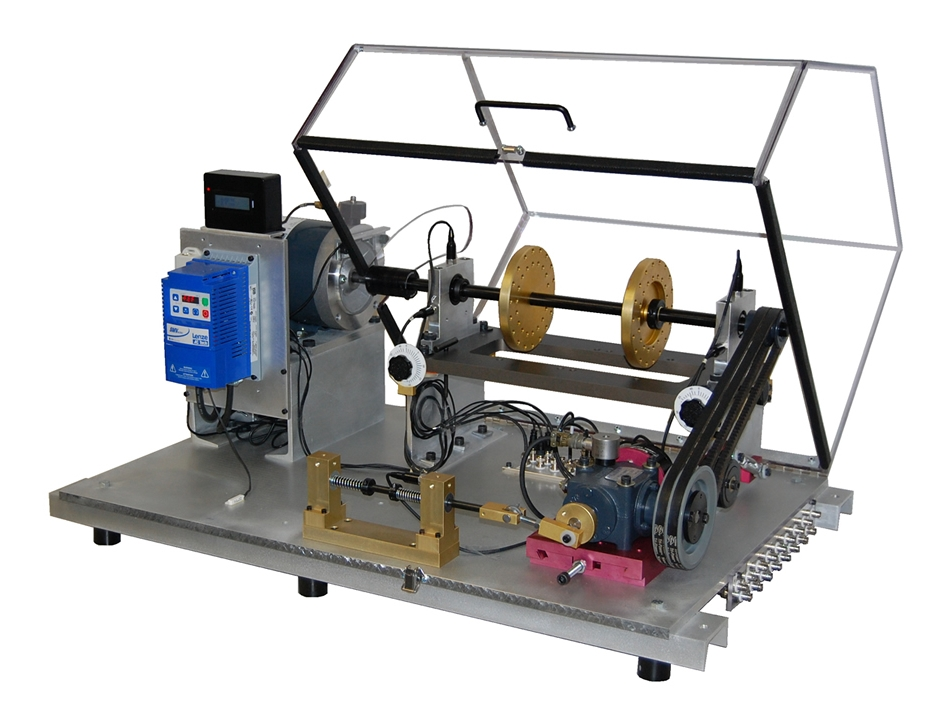
\includegraphics[width=0.7\textwidth]{assets/mafaulda-simulator.jpg}
\caption{SpectraQuest's Machinery Fault Simulator}
\label{fig:mafaulda-simulator}
\end{figure}

\begin{figure}[h]
\centering
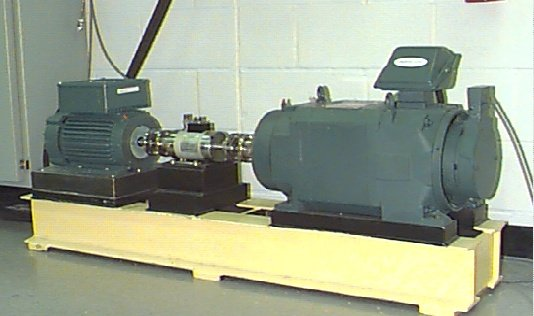
\includegraphics[width=0.7\textwidth]{assets/cwru-test-stand.jpg}
\caption{CWRU apparatus}
\label{fig:mafaulda-simulator}
\end{figure}

\begin{figure}[h]
\centering
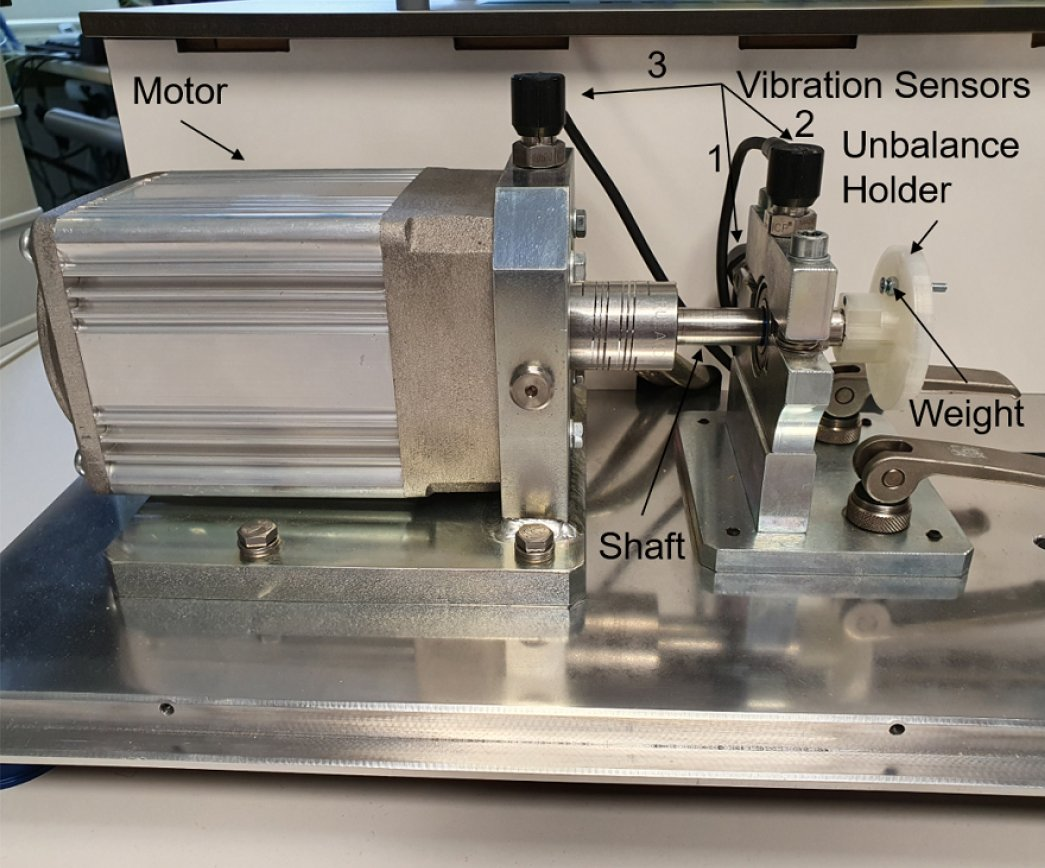
\includegraphics[width=0.7\textwidth]{assets/rotating-shaft.jpg}
\caption{Rotating shaft dataset}
\label{fig:rotating-shaft}
\end{figure}


\paragraph{CWRU}
2 HP (1.492 kW) Reliance Electric motor
Bearings - Inner, Outer
12 kHz, 48 kHz
fan and drive end bearings
Fault diameters of 7 mils, 14 mils, 21 mils, 28 mils, and 40 mils (1 mil=0.001 inches) in diameter were introduced separately at the inner raceway, rolling element (i.e. ball) and outer raceway. 
Faulted bearings were reinstalled into the test motor and vibration data was recorded for motor loads of 0 to 3 horsepower (motor speeds of 1797 to 1720 RPM).

% Feature-based performance of SVM and KNN classifiers for diagnosis of rolling element bearing faults
\cite{jamil_feature-based_2021}
% Machine Learning-Based Unbalance Detection of a Rotating Shaft Using Vibration Data
\cite{mey_machine_2020}

\paragraph{Rotating Shaft}
Shaft -  unbalances of different sizes
4 kHz

\section{Sensor and microcontroller}
% Intelligent Sensor Networks: The Integration of Sensor Networks, Signal Processing and Machine Learning
\cite{hu_intelligent_2012} 
